\documentclass[../poliXuniversity_hospital_-USP-report.tex]{subfiles}
\graphicspath{ {images/}{../images/}{../../images/} }

\begin{document}
%\clearpage
\chapter{Algoritmos de Controle}

\section{ROS}

%------------------------------------------
\begin{wrapfigure}{r}{5.5cm}
\centering
\caption{Framework ROS}\label{wrap-fig:1}

\includegraphics[width=6cm]{ros.jpeg}
\caption*{Fonte: Foto disponibilizada em ros.org}\label{wrap-fig:1}
\end{wrapfigure} 
%------------------------------------------

A sigla significa Robotic Operating System, no entanto, o ROS não é exatamente um sistema operacional. O ROS é um meta-sistema operacional, ou seja é uma coleção de frameworks,  voltado para o controle de robôs autônomos, que busca padronizar a forma como se organiza e se escreve código em robótica. Dessa forma, seguindo a ideia de padronizar com um conjunto s de convenções, é possível reutilizar códigos.

Em engenharia da computação, há a necessidade de padronizar códigos da mesma forma que na engenharia mecânica há a necessidade de padronizar parafusos. Por mais diferentes que possam ser dois robôs, existe uma série de atividades básicas e cotidianas que costumam aparecer em quase todos os projetos, como ler sensores, analisar e filtrar dados, acionar motores etc. Dessa forma, como uma série de pessoas usam a mesma convenção, a importação desse código se torna mais fácil e natural, assim, focar mais na unicidade do nosso robô do que uma série de implementações já feitas várias vezes.

\subsection{Funcionamento}
Como um todo, ROS facilita o tráfego de análise de informações, os seus principais conceitos podem ser vistos abaixo: 

\begin{itemize}
  \item Node: Menor unidade de processos executáveis, ou seja a unidade mínima de um projeto no ROS. Um node é um pedaço de código que realiza uma determinada tarefa. Cada node transmite e recebe informações por meio da message.
  \item Package: Principal unidade de organização do software no ROS e é composto de um ou mais nodes, informações para execução dos nodes, entre outros. O package é a menor unidade de construção e lançamento do ROS.
  \item Message: É a forma de comunicação entre os nodes. As messages possuem dados que fornecem informações para outros nodes. Um exemplo prático de message seria a leitura de um sensor de distância.
  \item Topic: Canal de comunicação entre nodes e identifica o conteúdo da message. Quando um node está enviando dados, dizemos que está publicando um topic, ou seja, ele é o publisher. Já quando um node está recebendo dados, ele está assinando um topic, ou seja, ele é o subscriber.
  \item Master: Núcleo do ambiente em ROS e sabe o que está acontecendo em todo o sistema. É responsável por inicializar o sistema e fornecer o registro de nomes e o serviço de pesquisa para os nodes. Além disso, ela também configura as conexões entre os nodes.
\end{itemize}

De maneira geral, tudo  repassado aqui tem como base o guia oficial de utilização do ROS \cite{ros_wiki21}, que é disponibilizado de graça.

\begin{figure}[h]
\centering
    \caption{Funcionamento do ROS}
    \centering % para centralizarmos a figura
    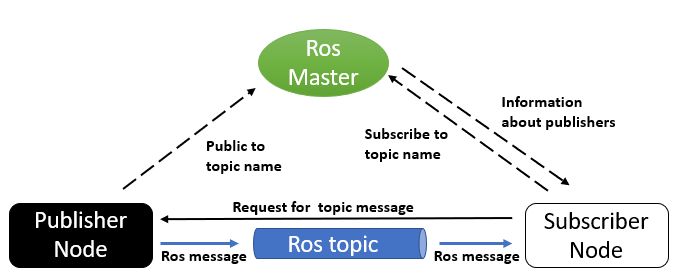
\includegraphics[width=14cm]{ros-concepts.png}
    \caption*{Fonte: Retirado de \cite{rosgazeboguide21}}
    \label{figura:1° Versão Robô Hospitalar}
\end{figure}

De certa forma, o que resta esclarecer é como é feita a integração dos algoritmos feitos em ROS com o simulador Gazebo.
Como o Gazebo faz parte dos Frameworks associados ao ROS, a integração entre os dois sistemas é muito simples. Todos os tópicos publicados no ROS podem ser lidos no Gazebo, dessa forma, somente exigindo que associemos um determinado tópico a algum link ou joint do nosso robô.

\section{Estrutura dos algoritmos}

Quando pensamos na construção do software de um robô autônomo, é quase que imediatamente associamos aos algoritmos que são executados e dados que são processados. Dessa forma, realizar tomadas de decisão e reagir da melhor forma possível a alguma adversidade do ambiente.

No caso do robô hospitalar não é diferente. Na estrutura geral do software do robô hospitalar a ideia é constituída, até o momento, basicamente: mapeamento do ambiente, planejamento global e local e uma odometria ainda em desenvolvimento. Além dessa, há uma parte muito importante de processamento de dados, o qual consiste em preparar os dados para enviar para os dispositivos embarcados, para assim realizar o envio da informação pela comunicação Serial \cite{ssh21}. Para saber mais sobre isso, verificar a seção de Comunicação com Embarcados.

\subsection{Mapeamento}

%------------------------------------------
\begin{wrapfigure}{r}{5.5cm}
\centering
\caption{RPLidar A1M8}\label{wrap-fig:1}
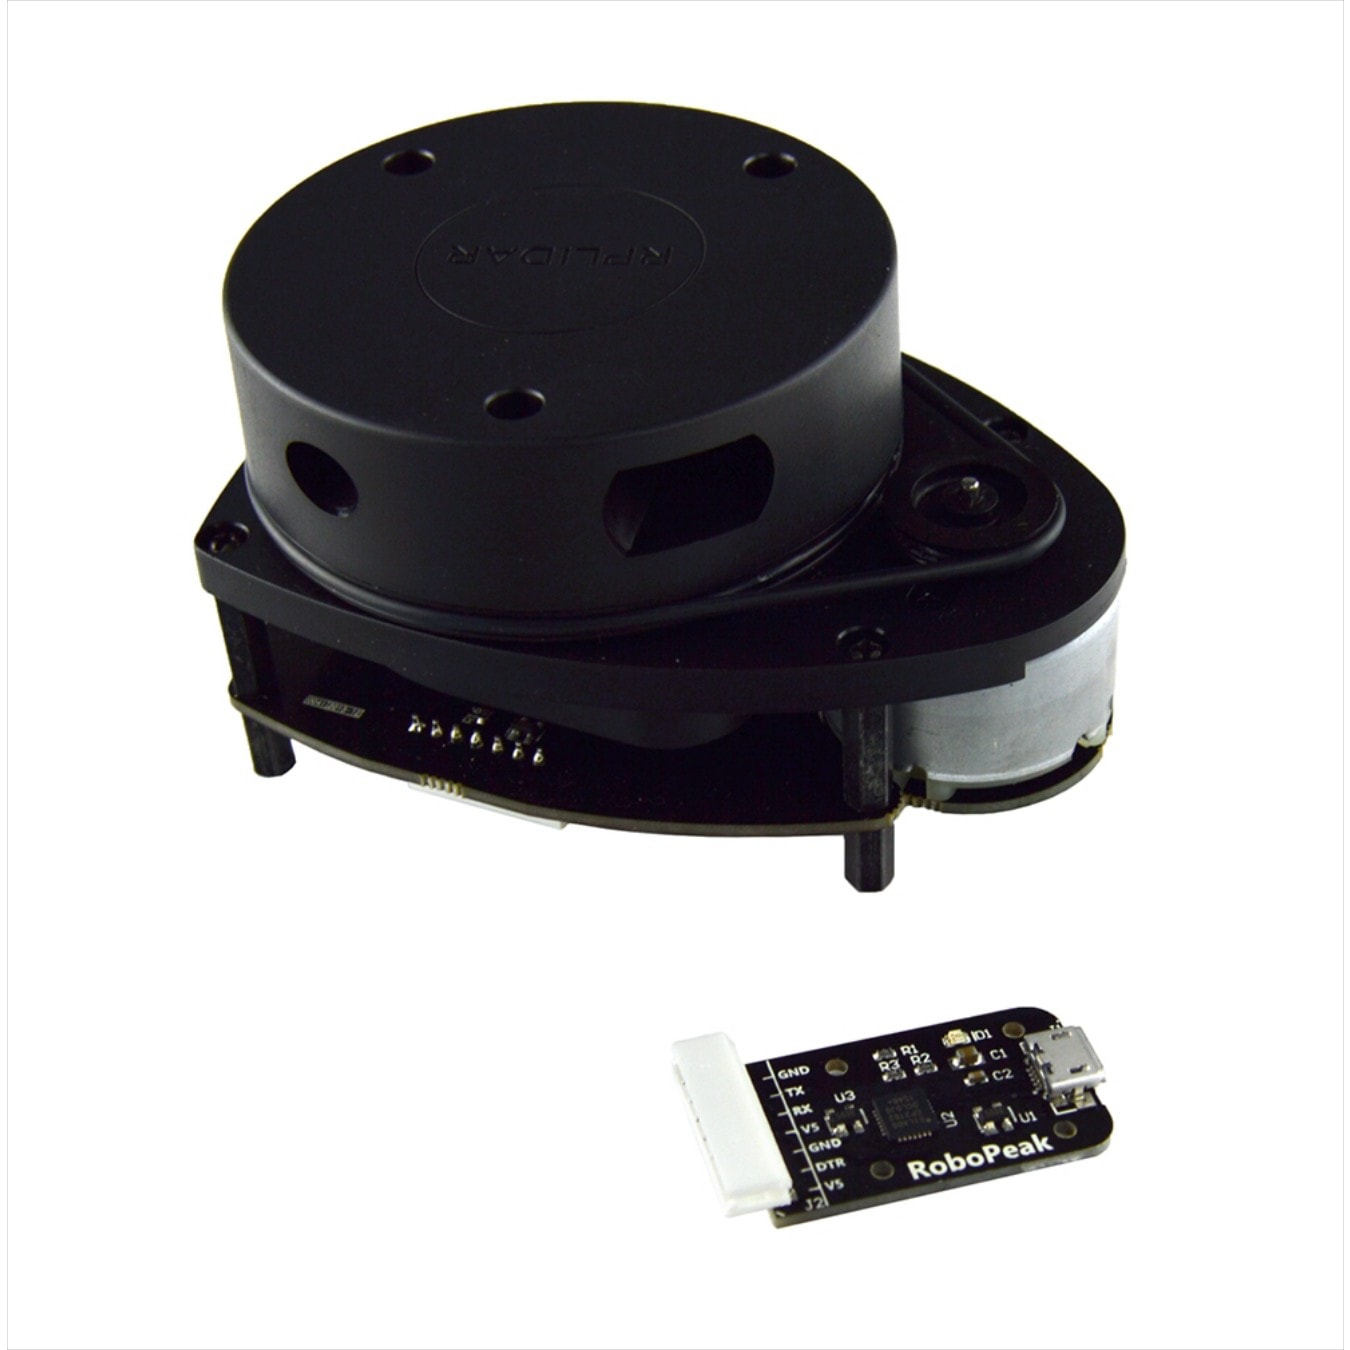
\includegraphics[width=4cm]{lidar_jetson.jpg}
\caption*{Fonte: Foto disponibilizada \cite{lidara121}}\label{wrap-fig:1}
\end{wrapfigure} 
%------------------------------------------

O robô, para definir a sua rota para determinado ponto do mapa precisa ter noção macro e micro do ambiente que ele se encontra. Para haver a possibilidade do robô ter essas noções é necessário haver o mapeamento do ambiente que o robô se encontra e deixar isso registrado em um mapa com formato suportado pelo ROS. 

Para realizar o mapeamento do ambiente, foi feitos teste com RPLidar A1M8 R6 \cite{lidara121} e 
Slamtec Mapper M1M1 \cite{lidarmapper21}, ambos lidares feitos para mapeamentos. Ambos tiveram bons resultados, porém o Mapper não tem suporte para arquitetura computacional da Jetson, então ele foi usado somente em computadores e dispositivos mobile.

\subsubsection{Mapas obtidos}

A partir de simulações usando o Rviz \cite{rviz21}, outro framework associado ao ROS, pudemos simular o mapeamento com o robô em um ambiente hospitalar. Simular o mapeamento no hospital simulado foi de extrema importância para o projeto, pois os integrantes do projeto não estavam permitidos a frequentar o laboratório na USP na época. o resultado pode ser vista na figura ~\ref{fig:Hospital Simulado Mapeado}.

\begin{figure}[!h]
\centering
    \caption{Hospital Simulado Mapeado}
    \centering % para centralizarmos a figura
    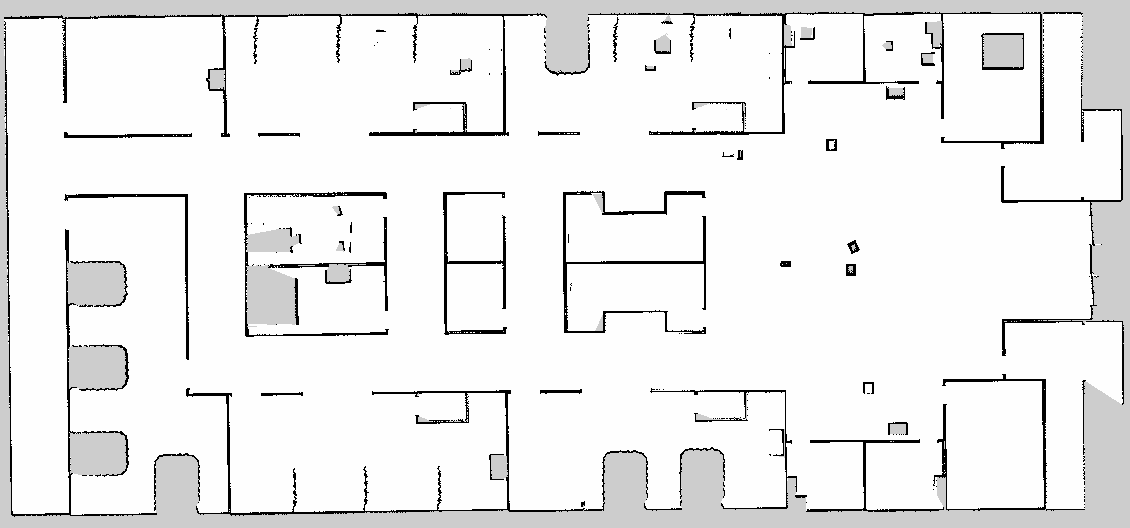
\includegraphics[width=12cm]{hospital_map.png}
    \caption*{Fonte: Elaborada pelo autor pelo Software Rviz \cite{rviz21}}
    \label{fig:Hospital Simulado Mapeado}
\end{figure}

Depois de simulado, foi realizado o mapeamento usando o lidar Mapper na casa de um dos integrantes do projeto. O resultado pode ser visto na figura ~\ref{fig:Mapeamento real -  teste}.

\begin{figure}[!h]
\centering
    \caption{Mapeamento real -  teste}
    \centering % para centralizarmos a figura
    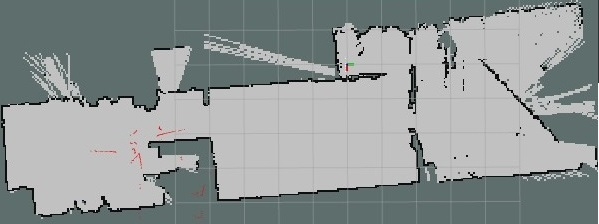
\includegraphics[width=14cm]{mapa_teste.jpeg}
    \caption*{Fonte: Elaborada pelo autor pelo Software Rviz \cite{rviz21}}
    \label{fig:Mapeamento real -  teste}
\end{figure}

\subsection{Navegação}

Depois que todo o mapeamento tiver sido feito, pode-se estimar uma posição inicial para o robô começar a se locomover e a partir dele o robô e ir estimando a sua posição com parâmetros da sua odometria. Entretanto, quando se pensa na navegação do robô, é preciso mensurar a todo momento a posição atual, com seu erro, e a rota que o robô vai prosseguir naquele momento. Por conta disso, foi implementado um algoritmo de localização e de planejamento de rotas.

\subsubsection{Localizacão}

Assim como na primeira versão do robô hospitalar, para localizar o robô no mapa o módulo foi utilizado o algoritmo de Adaptive Monte Carlo Localization \cite{amcl21}, que é mais conhecido como AMCL e já se encontra de forma nativa no ROS. Com esse algoritmo, podemos estimar a posição do robô e seus erros, que é indicado na figura ~\ref{fig:Adaptive Monte Carlo Localization}.

\begin{figure}[h]
\centering
    \caption{Adaptive Monte Carlo Localization \cite{amcl21},}
    \centering % para centralizarmos a figura
    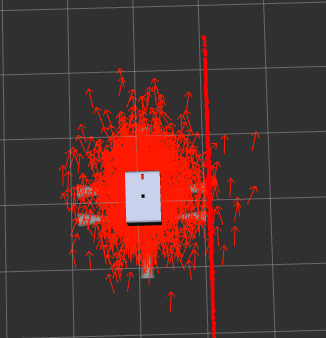
\includegraphics[width=10cm]{robo_posicao.png}
    \caption*{Fonte: Elaborada pelo autor no Software Rviz\cite{rivz21}}
    \label{fig:Adaptive Monte Carlo Localization}
\end{figure}

O algoritmo em questão trabalha junto a odometria, recebendo dados da posição do robô nos eixos x e y. A partir desses dados, gera uma nuvem probabilidade para robô estar, assim, conforme o robô se movimenta essa posição é corrigida e a nuvem de probabilidade diminui, o que indica a maior precisão da posição atual do robô. Na figura ~\ref{fig:Adaptive Monte Carlo Localization}, pode-se ver a nuvem de posições.

\subsubsection{Planejamento de Rotas}

Para gerar o mapa de custos e calcular a melhor rota possível foi utilizado o pacote Move Base  \cite{movebase21} , que assim como o AMCL \cite{amcl21}, é um algoritmo já implementado e nativo do próprio ROS. O funcionamento desse pacote do ROS pode ser visto a figura \ref{fig:Funcionamento do Move base}.

\begin{figure}[h]
\centering
    \caption{Funcionamento do Move base}
    \centering % para centralizarmos a figura
    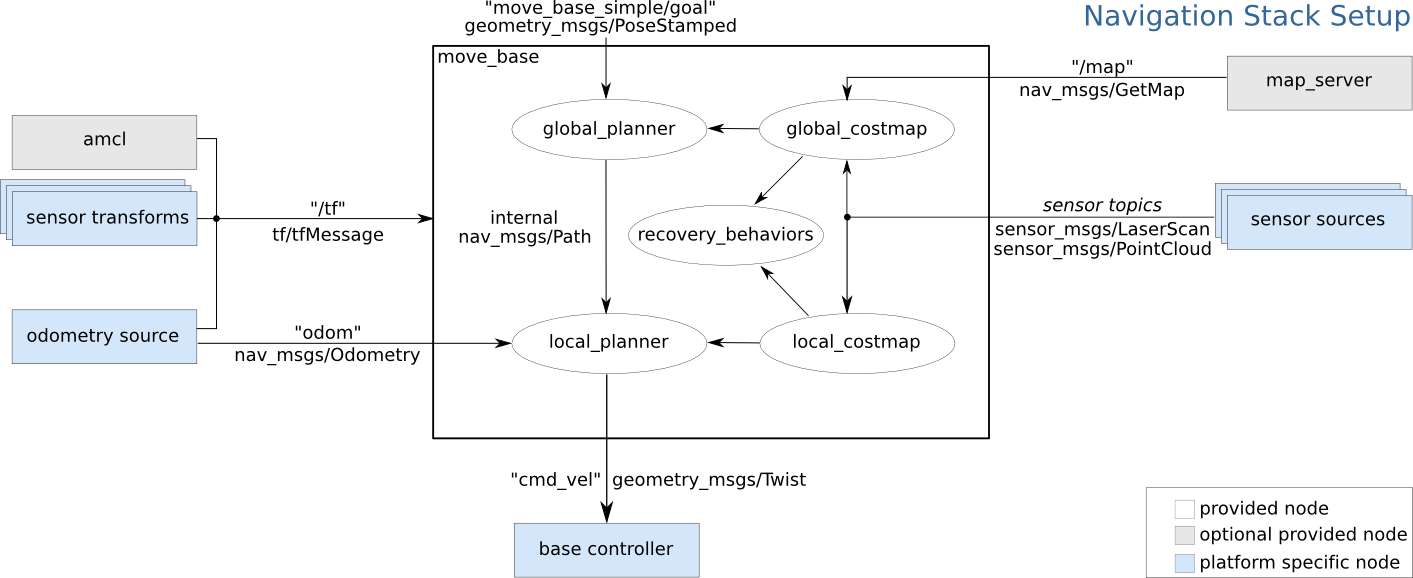
\includegraphics[width=14cm]{move_base.png}
    \caption*{Fonte: Retidada do ROS Wiki \cite{ros_wiki21}}
    \label{fig:Funcionamento do Move base}
\end{figure}

De maneira geral, o pacote move base fornece um auxílio para gerar rotas para robôs no geral para os usuários de ROS. Assim, o Algoritmo “emprestado” gera um escopo de um plano local e global para o definir a rota que o robô precisará traçar para chegar no local desejado.

Para o planejar a rota local, o algoritmo não leva em consideração os mapas gerados, mas sim os dados coletados por sensores de distância e pelo lidar. O principal objetivo de planejar uma rota local é evitar imprevistos, como alguém entrar na frente do robô ou colocar um objeto em um lugar que não tinha antes. Assim que houver a detecção de algum desses imprevistos, o robô calcula uma nova rota que não tenha esse obstáculo. Para realizar tal mudança, é gerado um mapa de custo local (local\_costmap). Vale ressaltar, que como é um plano que tem como função evitar problemas, ele está atualizando constantemente.

Graças ao Move Base, há uma série de parâmetros que se pode usar para configurar o mapa gerado usado e regular ele para atender melhor a estrutura do robô produzido. na figura ~\ref{fig:Planjamento de rota - Local} pode-se ver a rota local naquele ponto.

\begin{figure}[h]
\centering
    \caption{Planjamento de rota - Local}
    \centering % para centralizarmos a figura
    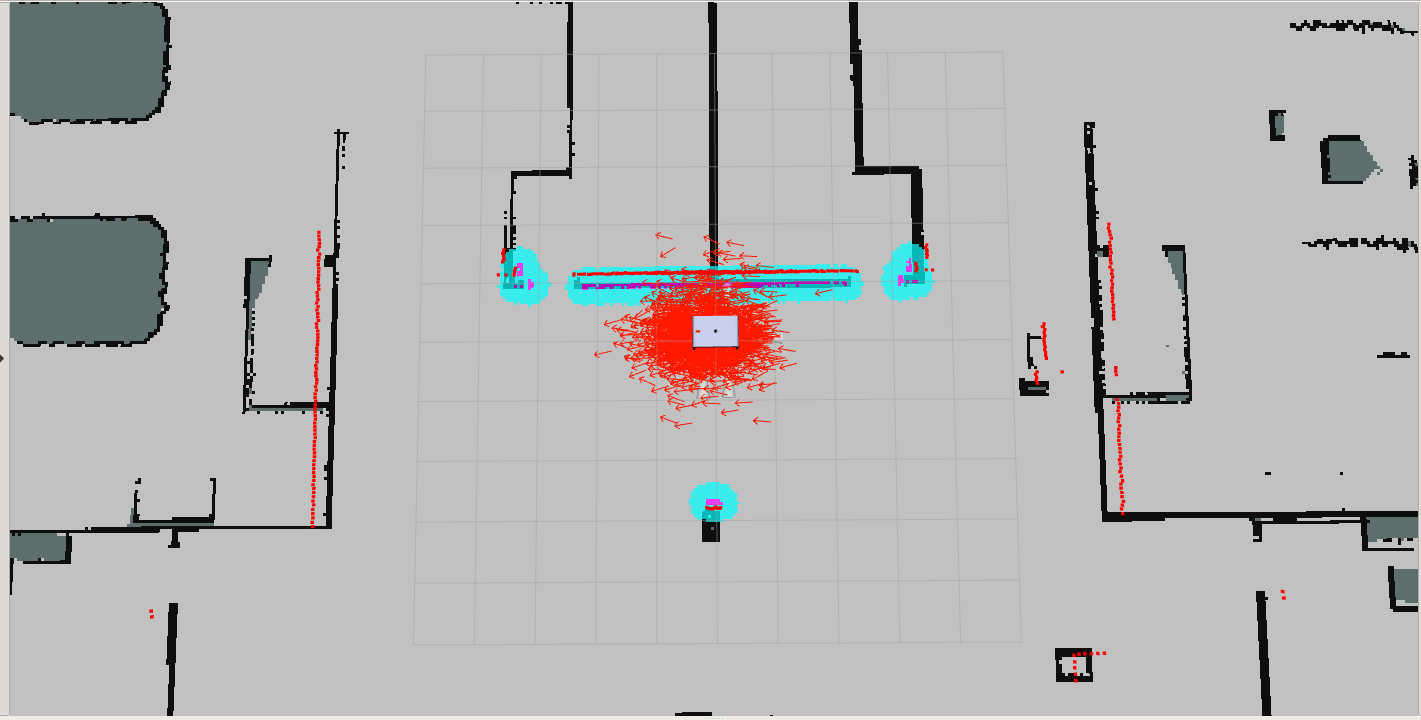
\includegraphics[width=12cm]{rota_local.png}
    \caption*{Fonte: Elaborada pelo autor no Software Rviz\cite{rivz21}}
    \label{fig:Planjamento de rota - Local}
\end{figure}

O mapa global, por outro lado, somente recebe o mapa do ambiente, e a partir de algoritmos nativos do ROS, calcula o mapa de custo global (global\_costmap) e define a melhor rota até determinado ponto. De maneira geral, o mapa consegue mensurar as áreas que o robô pode circular, as que ele deve evitar e as que ele não pode chegar perto, como paredes. Dessa forma, as regiões próximas às que são proibidas tendem a ser regiões a ser evitadas.

 O mapa de custo global, como um todo, se comporta como um campo escalar de duas dimensões, o qual as regiões proibidas tendem a ter um peso infinito e as regiões livres, peso zero. O peso da região tende a aumentar de forma exponencial conforme se aproxima da região proibida. No mapa de custo global gerado pelo próprio ROS, se pode alterar parâmetros do crescimento dessa exponencial para se adequar o melhor possível ao robô produzido. O mapa globa e a rota traçada podem ser visto na figura ~\ref{fig:Planjamento de rota - Global} e ~\ref{fig:Planjamento de rota - Tragetório}


\begin{figure}[h]
\centering
    \caption{Planjamento de rota - Global}
    \centering % para centralizarmos a figura
    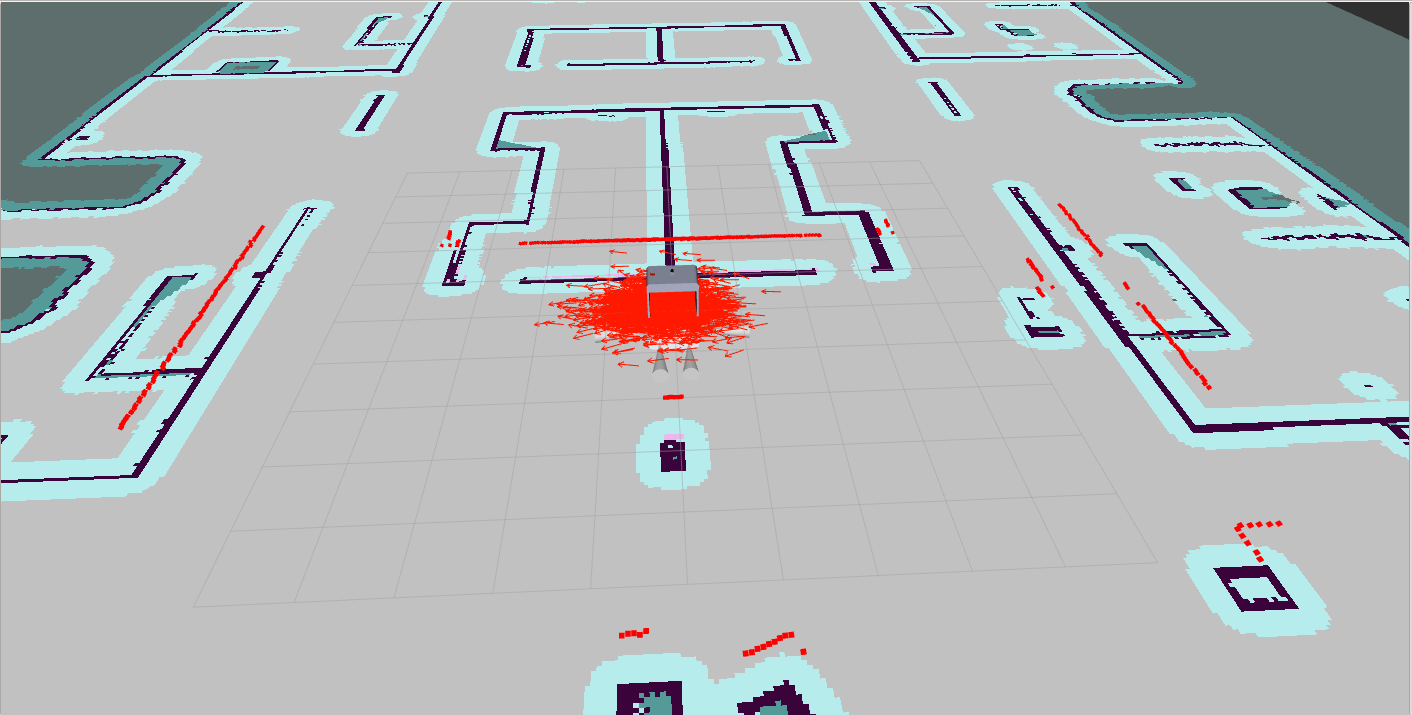
\includegraphics[width=12cm]{rota_global.png}
    \caption*{Fonte: Elaborada pelo autor no Software Rviz\cite{rivz21}}
    \label{fig:Planjamento de rota - Global}
\end{figure}

\begin{figure}[h]
\centering
    \caption{Planjamento de rota - Tragetório}
    \centering % para centralizarmos a figura
    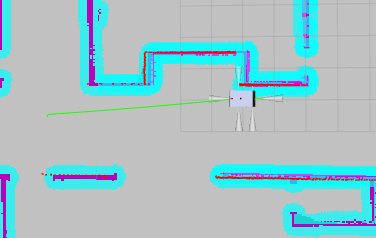
\includegraphics[width=15cm]{robo_rota2.png}
    \caption*{Fonte: Elaborada pelo autor no Software Rviz\cite{rivz21}}
    \label{fig:Planjamento de rota - Tragetório}
\end{figure}

\end{document}